\chapter{Brief history of data science}
\label{chap:history}

\chapterprecishere{``Begin at the beginning,'' the King said gravely, ``and
go on till you come to the end: then stop.''\par\raggedleft--- \textup{Lewis
Carroll}, Alice in Wonderland}

There are many points-of-view about the beginning of data science.  For the sake of
contextualization, I separate the topic in two approaches: the history of the term itself
and a broad timeline of data-driven sciences highlighting the important figures in each
age.

\begin{mainbox}{Chapter remarks}
  \boxsubtitle{Context}

  \begin{itemize}
    \item The term ``data science'' is recent and has been used to label rather different fields.
    \item The history of data-driven sciences is long and rich.
  \end{itemize}

  \boxsubtitle{Objectives}

  \begin{itemize}
    \item Understand the history of the term ``data science.''
    \item Understand the history of data-driven sciences.
  \end{itemize}

  \boxsubtitle{Takeways}

  \begin{itemize}
    \item There is no consensus on the definition of data science.
    \item There is enough evidence to support data science as a new science.
  \end{itemize}
\end{mainbox}

\section{The term ``data science''}

The term data science is recent and has been used to label rather different fields of
study.  In the following, I emphasize the history of a few notable usage of the term.

\def\naurds{(0,0) circle (20mm)}
\def\naurcs{(0:5mm) circle (15mm)}
\def\naurde{(0:40mm) circle (15mm)}

\colorlet{circle edge}{black!50}
\colorlet{circle area}{black!20}

\tikzset{filled/.style={fill=circle area, draw=circle edge, thick},
    outline/.style={draw=circle edge, thick}}

\begin{figure}
  \centering
  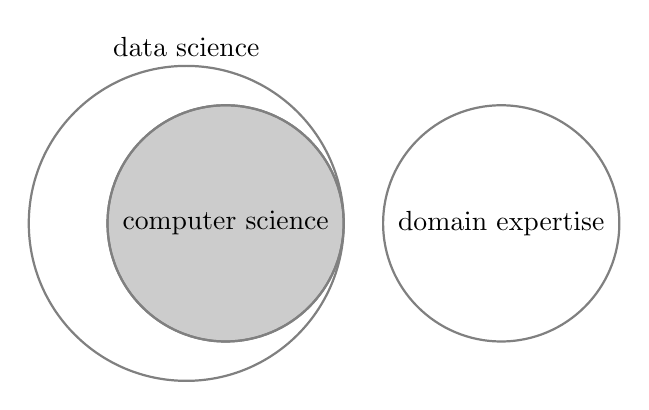
\begin{tikzpicture}
    \begin{scope}
      \clip \naurds;
      \fill[filled] \naurcs;
    \end{scope}
    \draw[outline] \naurds node(ds) {};
    \draw[outline] \naurcs node {computer science};
    \draw[outline] \naurde node {domain expertise};
    \node[anchor=north,above] at (0,2) {data science};
  \end{tikzpicture}
  \caption{
    Naur's view of data science.  For him, data science studies the techniques to deal
    with data, but he delegates the meaning of data to other fields.
  }
  \label{fig:naur}
\end{figure}

\paragraph{Peter Naur (1928 -- 2016)}

The term ``data science'' itself was coined in the 1960s by Peter Naur (/naʊə/). Naur was
a Danish computer scientist and mathematician who made significant contributions to the
field of computer science, including his work on the development of programming
languages\footnote{He is best remembered as a contributor, with John Backus, to the
Backus–Naur form (BNF) notation used in describing the syntax for most programming
languages.}.
His ideas and concepts laid the groundwork for the way we think about programming and data
processing today.

\begin{mainbox}{Peter Naur}
  \begin{itemize}
    \item Danish computer scientist and mathematician.
    \item Coined the term ``data science'' in the 1960s.
    \item Proposed the term ``datalogy'' as an alternative to computer science.
  \end{itemize}
\end{mainbox}

Naur disliked the term computer science and suggested it be called datalogy or data
science.  In the 1960s, the subject was practised in Denmark under Peter
Naur's term datalogy, which means the science of data and data processes.

He coined this term to emphasize the importance of data as a fundamental component of
computer science and to encourage a broader perspective on the field that included
data-related aspects. At that time, the field was primarily centered on programming
techniques, but Naur's concept broadened the scope to recognize the intrinsic role of data
in computation.

In his book\footnote{Peter Naur: Concise Survey of Computer Methods, 397 p.
Studentlitteratur, Lund, Sweden, ISBN 91-44-07881-1, 1974.
\url{http://www.naur.com/Conc.Surv.html}}, ``Concise Survey of Computer Methods'', he
parts from the concept that \emph{data} is ``a representation of facts or ideas in a
formalised manner capable of being communicated or manipulated by some
process.''\footnote{I. H. Gould (ed.): ‘IFIP guide to concepts and terms in data
processing’, North-Holland Publ. Co., Amsterdam, 1971.} Note however that his view of the
science only ``deals with data [\dots] while the relation of data to what they represent
is delegated to other fields and sciences.''

\def\clevelandds{(0,0) circle (20mm)}
\def\clevelandst{(0:-5mm) circle (15mm)}
\def\clevelandde {(2,1) circle (15mm)}
\def\clevelandcs {(2,-1) circle (15mm)}

\begin{figure}
  \centering
  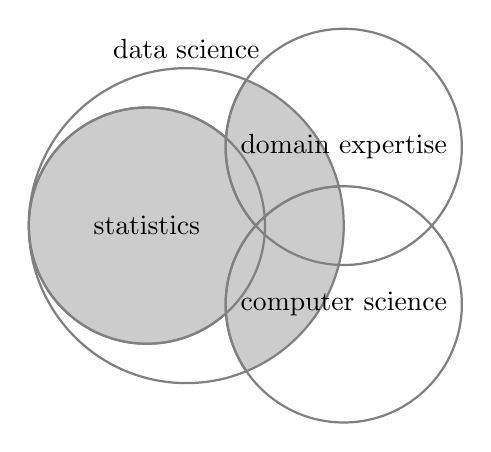
\begin{tikzpicture}
    \begin{scope}
      \clip \clevelandds;
      \fill[filled] \clevelandst;
      \fill[filled] \clevelandde;
      \fill[filled] \clevelandcs;
    \end{scope}
    \draw[outline] \clevelandds node(ds) {};
    \draw[outline] \clevelandst node {statistics};
    \draw[outline] \clevelandde node {domain expertise};
    \draw[outline] \clevelandcs node {computer science};
    \node[anchor=north,above] at (0,2) {data science};
  \end{tikzpicture}
  \caption{
    Cleveland's view of data science.  For him, data science is the ``modern'' statistics,
    where it is enlarged by computer science and domain expertise.
  }
  \label{fig:cleveland}
\end{figure}

\paragraph{William Cleveland (born 1943)}

In 2001, a prominent statistician used the term ``data science" in his work to describe a
new discipline that comes from his ``plan to enlarge the major areas of technical work of
the field of statistics\footnote{W. S. Cleveland. Data Science: An Action Plan for
Expanding the Technical Areas of the Field of Statistics. ISI Review, 69:21–26, 2001.}.''
In 2014, that work was republished\footnote{W. S. Cleveland.
Data Science: An Action Plan for the Field of Statistics. Statistical Analysis and Data
Mining, 7:414–417, 2014. reprinting of 2001 article in ISI Review, Vol 69.}.
He advocates the expansion of statistics beyond theory into technical areas, significantly
changing statistics.  Thus, it warranted a new name.

\begin{mainbox}{William Cleveland}
  \begin{itemize}
    \item American statistician.
    \item Proposed the discipline ``data science'' in 2001.
    \item Proposed the term ``data science'' as the new name for expansion of statistics.
  \end{itemize}
\end{mainbox}

As a result, William Swain Cleveland II is credited to define data science as it is most
used today. He is a highly influential figure in the fields of statistics, machine
learning, data visualization, data analysis for multidisciplinary studies, and high
performance computing for deep data analysis.

\paragraph{Buzzword or a new science?}

Be aware that literature has no consensus on the definition of data science, and it is still considered
by some to be a buzzword\footnote{Press, Gil. "Data Science: What's The Half-Life of a
Buzzword?". Forbes. Available at
\url{https://www.forbes.com/sites/gilpress/2013/08/19/data-science-whats-the-half-life-of-a-buzzword/}}.

Most of the usages of the term in literature and in the media are either a rough
reference to a set of data-driven techniques or a marketing strategy.  Naur
(\cref{fig:naur}) and Cleveland (\cref{fig:cleveland}) are among the few that try to
carefully define the term.  However, both of them do not see data science as an
independent field of study, but an enlarged scope of an existing science.  I disagree;
the social and economical demand for data-driven solutions led to an evolution in our
understanding of the challenges we are facing.  As a result, we see many ``data
scientist'' being hired and many ``data science degrees'' programs emerging.

In \cref{chap:data}, I dare to provide a (yet another) definition for the term.  I
argue that its object of study can be precisely established to support it as a new
science.

\begin{mainbox}{A new science}
  \begin{itemize}
    \item Both Naur and Cleveland do not see data science as an independent field of study.
    \item I argue that data science is not a buzzword.
    \item Our social and economical reality demands a new science.
  \end{itemize}
\end{mainbox}

\section{Timeline and historical markers}

\textcite{Kelleher2018} provides an interesting time line of data-driven methods and
influential figures in the field.  I reproduce it here with some minor changes, including
some omissions and additions.

Like \citeauthor{Kelleher2018}, I address data collection, and then data analysis.

\subsection{Timeline of data collection}

The importance of collecting data goes without saying.  Data fuels analysis and
decision making.  In the following, I present some of the most important milestones in the history
of data collection.

\begin{figure}
  \centering
  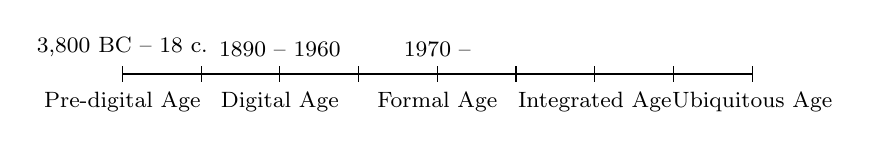
\begin{tikzpicture}
    \draw (0,0) -- (8,0);
    \foreach \x in {0,1,...,8} {
      \draw (\x,-0.1) -- (\x,0.1);
    }
    \foreach \x/\y/\z in {%
        0/Pre-digital Age/{3,800 BC -- \nth{18} c.},
        2/Digital Age/{1890 -- 1960},
        4/Formal Age/{1970 --},
        6/Integrated Age/{},
        8/Ubiquitous Age/{}} {
      \node[anchor=north] at (\x,-0.1) {\footnotesize\y};
      \node[anchor=south] at (\x,0.1) {\footnotesize\z};
    }
  \end{tikzpicture}
  \caption{
    Timeline of the ages of data collection.
  }
  \label{fig:collection-history}
\end{figure}

\Cref{fig:collection-history} illutrates the timeline.

\subsubsection{Pre-digital age}

We can consider the earliest records of data collection to be the notches on sticks and
bones to keep tracking of passing of time.  The Lebombo bone, a baboon fibula with
notches, is probably the earliest known mathematical object.  It was found in the Lebombo
Mountains located between South Africa and Eswatini.
They estimate it is more
than 40,000 years old. It is conjectured to be a tally stick, but its exact purpose is
unknown. Its 29 notches suggests that may have been used as a lunar phase counter.
However, since it is broken at one end, the 29 notches may or may not be the total
number\footcite{Beaumont2013}.

Another important milestone in the history of data collection is the record of
demographic data.  One of first known census was conducted in 3,800 BC in the Babylonian
Empire.  It was ordered to assess the population and resources of
his empire.  Records were stored on  clay  tiles\footcite{Grajalez2013}.

Since the early forms of writing, humanity abilities to record events and information
increased significantly.  The first known written records date back to around 3,500 BC, the
Sumerian archaic (pre-cuneiform) writing.  This writing system was used to represent
commodities using clay tokens and to record transactions\footcite{Ifrah1998}.

``Data storage'' was also a challenge.  Some important devices that increased our capacity
to register textual information are the Sumerian clay tablets (3,500 BC), the Egyptian
papyrus (3,000 BC), the Greek alphabet (800 BC), the Roman wax tablets (100 BC), the codex
(100 AD), the Chinese paper (200 AD), the printing press (1440), the typewriter (1868).

% Talvez citar na parte de análise de dados
% Other mechanisms were also developed to store information in a more structured way.  Some
% important devices are
% the abacus (2,700 BC), the Antikythera mechanism (150 -- 100 BC), the
% Chinese South Pointing Chariot (260 AD), the Pascaline (1642), the Jacquard loom (1801),
% the Babbage Difference Engine (1822), the Babbage Analytical Engine (1837).

Besides those improvements in unstructured data storage, at least in the Western and
Middle Eastern world, there are no significant advances in structured data collection
until the \nth{19} century.  (A Eastern timeline research is pending.)

I consider a major influential figure in the history of data
collection to be Florence Nightingale (1820 -- 1910).  She was a passionate statistician
and probably the first person to use statistics to influence public and official
opinion.  The meticulous records she kept during the Crimean War
(1853 -- 1856) were the evidence that saved lives.  She was also the first to use
statistical graphics to present data in a way that was easy to understand.  She is
credited with developing a form of the pie chart now known as the polar area
diagram.  She also reformed healthcare in the United Kingdom and
is considered the founder of modern nursing\footcite{Grajalez2013}.

\begin{mainbox}{Florence Nightingale}
  \begin{itemize}
    \item Passionate statistician.
    \item First person to use statistics to influence public and official opinion.
    \item Organized data from garden fruits and vegetables into numerical tables at the age of 9.
    \item At 20 she was receiving two-hour lessons from a Cambridge-trained mathematician.
    \item She found the sight of a long column of figures ``perfectly reviving.''
    \item She went out to the Crimean War, to Scutari in Turkey, in 1854.
    \item She found that not even the numbers of soldiers entering the hospitals, or leaving them – alive or dead – was known.
    \item From the first she kept meticulous records.
    \item The data she collected was the evidence that saved lives.
    \item She was the first to use statistical graphics to present data in a way that was easy to understand.
    \item She is credited with developing a form of the pie chart now known as the polar area diagram.
    \item She reformed healthcare in the United Kingdom and is considered the founder of modern nursing.
  \end{itemize}
\end{mainbox}

\begin{mainbox}{Pre-digital age}
  \begin{itemize}
    \item Babylonian census (3,800 BC)
    \item Sumerian archaic (pre-cuneiform) writing (3,500 BC)
    \item Egyptian papyrus (3,000 BC)
    \item Phoenician alphabet (1,000 BC)
    \item Greek alphabet (800 BC)
    \item Roman wax tablets (100 BC)
    \item Codex (100 AD)
    \item Chinese paper (200 AD)
    \item Printing press (1440)
    \item Typewriter (1868)
    \item Florence Nightingale (1820 -- 1910)
  \end{itemize}
\end{mainbox}

\subsubsection{Digital age}

In the modern period, several devices were developed to store digital\footnote{Digital
means the representation of information in (finite) discrete form.  The term comes from the Latin
digitus, meaning finger, because it is the natural way to count using fingers.}
information.  One particular device that is important for data collection is the punched
card.  It is a piece of stiff paper that contains digital information represented by the
presence or absence of holes in predefined positions.  The information can be read by a
mechanical or electrical device called a card reader.  The earliest famous usage of
punched cards was by Basile Bouchon (1725) to control looms.  Most of the advances until
the 1880s were about the automation of machines using hand-punched cards, and not
particularly specialized for data collection.

However, the 1890 census in the United States was the first to use machine-readable
punched cards to tabulate data. Processing 1880 census data took eight years, so the
Census Bureau contracted Herman Hollerith (1860 -- 1929) to design and build a tabulating
machine.  He founded the Tabulating Machine Company in 1896, which later merged with other
companies to become International Business Machines Corporation (IBM) in 1924. Later
models of the tabulating machine were widely used for business applications such as
accounting and inventory control. Punched card technology remained a prevalent method of
data processing for several decades until more advanced electronic computers were
developed in the mid-\nth{20} century.

The invention of the digital computer is responsible for a revolution in data collection.
The amount of information we can capture and store increased exponentially.  ENIAC (1945) was
the first electronic general-purpose computer.  It was Turing-complete, digital, and
capable of being reprogrammed to solve a full range of computing problems.
It had 20 words of internal memory, each capable of storing a 10-digit decimal integer number.
Programs and data were entered by setting switches and inserting punched cards.

For the 1950 census, the United States Census Bureau used the
UNIVAC I (Universal Automatic Computer I), the first commercially produced computer in the
United States\footnote{Read more in \url{https://www.census.gov/history/www/innovations/}.}.

It goes without saying that digital computers have become much more powerful and
sophisticated since then.  The data collection process has been easily automated and
scaled to a level that was unimaginable before.  However, ``where'' storing data is
not the only challenge.  ``How'' to store data is also a challenge.  The next period of
history addresses this issue.

\begin{mainbox}{Digital age}
  \begin{itemize}
    \item Punched card (1725)
    \item 1890 census and Hollerith's tabulating machine (1890)
    \item ENIAC (1945)
    \item UNIVAC I used by the United Census Bureau (1950)
  \end{itemize}
\end{mainbox}

\subsubsection{Formal age}

In 1970, Edgar Frank Codd (1923 -- 2003) published a paper entitled ``A Relational Model
of Data for Large Shared Data Banks''\footcite{Codd1970}.  In this paper, he introduced
the concept of a relational model for database management {\color{red}
provide more details}.

\subsection{Timeline of data analysis}

\begin{itemize}
  \item Summary statistics
  \item Probability Advent 17, 18th
  \item Statistical learning 19th
    \begin{itemize}
      \item Bayes rule
      \item Gauss’ method of least squares
      \item Playfair data visualization
    \end{itemize}
  \item 20th inference
    \begin{itemize}
      \item Pearson hypothesis testing
      \item Fisher multivariate analysis, maximum likelihood estimate
    \end{itemize}
  \item Computer: McCulloch Pitts, Shannon information theory, Fix and Hodged discriminatory analysis, knn
  \item Machine learning: 1965 Nils Nilsson neural network, 1966 Hunt inducing trees, Kmeans, Vapnik 71
  \item Today: Ensembles, Deep learning: vision and language, KDD
\end{itemize}
